\section{検証}
\subsection{RSA暗号を用いた検証}
整数論に関する関数はRSA暗号の計算を用いて,Rubyのみで計算する場合とmaplerubyで計算した場合でどのような差があるか検証する.検証のために以下のようなプログラムを用意した.
\begin{lstlisting}[style=customRuby,basicstyle={\scriptsize\ttfamily}]
#rsa_org.rb
require 'prime'
include Math

def rsa(input)
  c = input.to_i
  print "平文>>> #{c}\n"
  
  big_num = sqrt(c).to_i
  num = 1000
  
  p,q,n=0,0,0
  p = Prime.each.find{|e| e >= rand(big_num+1..big_num+num)}
  q = Prime.each.find{|e| e >= rand(big_num+1..big_num+num)}
  
  n = p*q
  l = (p-1).lcm(q-1)
  
  print "素数 p >>> #{p}\n"
  print "素数 q >>> #{q}\n"
  print "N >>> #{n}\n"
  print "L >>> #{l}\n"
  
  for e in 2..l do
    break if e.gcd(l)==1
  end
  
  print "公開鍵>>> E = #{e}, N = #{n}\n"
  
  for d in 2..l do
    break if (e*d)%l==1
  end
  
  print "秘密鍵>>> D = #{d}, N = #{n}\n"
  
  m = c**e % n
  re_c = m**d % n
  
  print "暗号化>>> #{m}\n"
  print "復号化>>> #{re_c}\n"
end

rsa(ARGV[0])
\end{lstlisting}
このプログラムはRubyだけで書かれている.例えば平文を256と入力すると,
\begin{lstlisting}[style=,basicstyle={\scriptsize\ttfamily}]
/Users/eri/mapleruby/lib% ruby rsa.rb 256
平文>>> 256
素数 p >>> 107
素数 q >>> 83
N >>> 8881
L >>> 4346
公開鍵>>> E = 3, N = 8881
秘密鍵>>> D = 1449, N = 8881
暗号化>>> 1007
復号化>>> 256
\end{lstlisting}
このような形で,出力してくれる.

\subsubsection{RSA暗号とは}
RSA暗号は桁数が大きい合成数の素因数分解問題が困難であることを安全性の根拠とした公開鍵暗号の1つである.
1977年に発明され,発明者であるロナルド・リベスト(Ron Rivest),アディ・シャミア(Adi Shamir),
レオナルド・エーデルマン(Len Adleman)ら3人のFamily nameの頭文字をつなげてこのように呼ばれている\cite{listings2}.
アルゴリズムは,

\begin{itemize}
\item p, q: 任意の素数.
\item N: p, qをかけた数.
\item L: p - 1とq - 1の最小公倍数.
\item E(Encryption exponent, 暗号化指数): Lと互いに素な数.Lとの最大公約数が1となる数.
\item D(Decryption exponent, 復号化指数): E*D mod L = 1となる数.
\end{itemize}
以上6つの値を用いて,平文を暗号化していく.
ここでの数Eと数Nのペアが公開鍵,数Dと数Nのペアが秘密鍵となる.
平文を暗号化する際は,
\begin{quote}\begin{verbatim}
 平文^E mod N (平文をE乗してNで割った余り)
\end{verbatim}\end{quote}
を行い,逆に復号化する際は,
\begin{quote}\begin{verbatim}
 暗号文^D mod N (暗号文をD乗してNで割った余り)
\end{verbatim}\end{quote}
を行う.

\subsubsection{Rubyのみで計算した場合}
Rubyのみで計算した場合,このプログラムでは,平文が1000000を越えたあたりから正しく出力ができなかったり数が大きすぎて計算ができないということが起こる.下記は平文が2000000だった場合の結果である.
\begin{lstlisting}[style=,basicstyle={\scriptsize\ttfamily}]
/Users/eri/mapleruby/lib% ruby rsa_org.rb 2000000
平文>>> 2000000
素数 p >>> 1459
素数 q >>> 1493
N >>> 2178287
L >>> 1087668
公開鍵>>> E = 5, N = 2178287
秘密鍵>>> D = 652601, N = 2178287
rsa_org.rb:36: warning: in a**b, b may be too big
暗号化>>> 1481122
復号化>>> NaN
\end{lstlisting}
\subsubsection{maplerubyを使った場合}
まず先ほどのrsa\_org.rbをmaplerubyを用いたrsa.rbに書き換えた.
\begin{lstlisting}[style=customRuby,basicstyle={\scriptsize\ttfamily}]
#rsa.rb
require './mapleruby'
include Math

def rsa(input)
  c = input.to_i
  print "平文>>> #{c}\n"
  
  big_num = sqrt(c).to_i
  num = 1000
  
  p,q,n=0,0,0
  p = RMaple.new.nextprime(rand(big_num+1..big_num+num))
  q = RMaple.new.nextprime(rand(big_num+1..big_num+num))
  
  n = p*q
  l = RMaple.new.lcm(p-1,q-1)
  
  print "素数 p >>> #{p}\n"
  print "素数 q >>> #{q}\n"
  print "N >>> #{n}\n"
  print "L >>> #{l}\n"
  
  for e in 2..l do
    break if RMaple.new.gcd(e,l)==1
  end
  
  print "公開鍵>>> E = #{e}, N = #{n}\n"
  
  d = Mapleruby.new("eval(1/#{e} mod #{l})").exec_i
  
  print "秘密鍵>>> D = #{d}, N = #{n}\n"
  
  x = Mapleruby.new("#{c}^#{e}").exec_i
  m = RMaple.new.mod(x, n)
  
  re_c = Mapleruby.new("#{m}^#{d} mod #{n}").exec_i
  
  print "暗号化>>> #{m}\n"
  print "復号化>>> #{re_c}\n"
end

rsa(ARGV[0])
\end{lstlisting}
このプログラムに関しては,maplerubyのrand関数では乱数が同じ値になって計算がうまくいかなくなるためRubyのrand関数を使用している.
rsa.rbを使った場合は,1000000000までの暗号化が可能であると分かった.
\begin{lstlisting}[style=,basicstyle={\scriptsize\ttfamily}]
/Users/eri/mapleruby/lib% ruby rsa.rb 1000000000
平文>>> 1000000000
{:MAPLE_PATH=>"/Library/Frameworks/Maple.framework/Versions/Current/bin/maple"}
31699
{:MAPLE_PATH=>"/Library/Frameworks/Maple.framework/Versions/Current/bin/maple"}
31657
{:MAPLE_PATH=>"/Library/Frameworks/Maple.framework/Versions/Current/bin/maple"}
167238648
素数 p >>> 31699
素数 q >>> 31657
N >>> 1003495243
L >>> 167238648
{:MAPLE_PATH=>"/Library/Frameworks/Maple.framework/Versions/Current/bin/maple"}
2
{:MAPLE_PATH=>"/Library/Frameworks/Maple.framework/Versions/Current/bin/maple"}
3
{:MAPLE_PATH=>"/Library/Frameworks/Maple.framework/Versions/Current/bin/maple"}
4
{:MAPLE_PATH=>"/Library/Frameworks/Maple.framework/Versions/Current/bin/maple"}
1
公開鍵>>> E = 5, N = 1003495243
{:MAPLE_PATH=>"/Library/Frameworks/Maple.framework/Versions/Current/bin/maple"}
秘密鍵>>> D = 100343189, N = 1003495243
{:MAPLE_PATH=>"/Library/Frameworks/Maple.framework/Versions/Current/bin/maple"}
{:MAPLE_PATH=>"/Library/Frameworks/Maple.framework/Versions/Current/bin/maple"}
96903649
{:MAPLE_PATH=>"/Library/Frameworks/Maple.framework/Versions/Current/bin/maple"}
暗号化>>> 96903649
復号化>>> 1000000000
\end{lstlisting}\begin{description}
\item[MAPLE\_PATHの文章のところでmaplerubyが動いている.
]\end{description}
\subsection{行列での検証}
まず,以下のようなプログラムを作った.
\begin{lstlisting}[style=customRuby,basicstyle={\scriptsize\ttfamily}]
require './mapleruby'

a = 3
b = 3
c = [[1,2,1],[4,5,6],[7,8,9]]

p x = RMaple.new.matrix(a, b, c)

p RMaple.new.matrixinverse(x)
p RMaple.new.eigenvectors(x)
\end{lstlisting}
これは3行3列の行列を生成したのち,それの逆行列と固有値・固有ベクトルを出力するプログラムである.これを実行すると図9のようになる.

\begin{figure}[htbp]\begin{center}
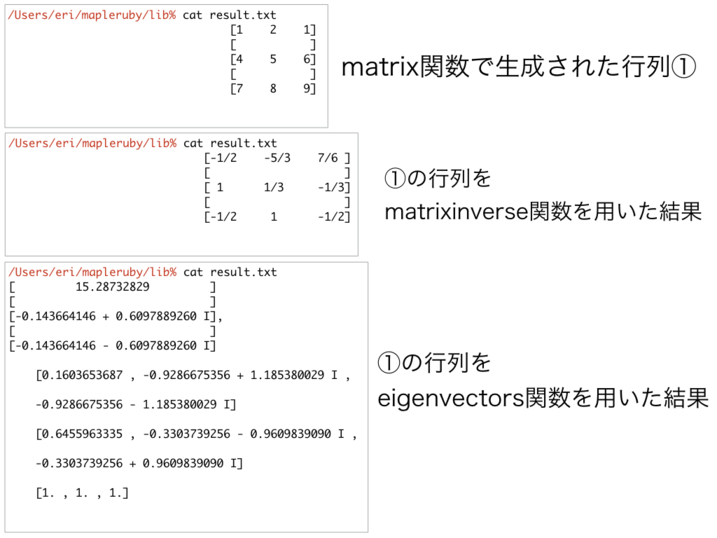
\includegraphics[width=10cm,bb= 0 0 737 553]{../figs/./mapleruby_eringi.008.png}
\caption{プログラムの出力結果}
\label{default}\end{center}\end{figure}
これと同じものをMapleで計算すると図10のようになる.

\begin{figure}[htbp]\begin{center}
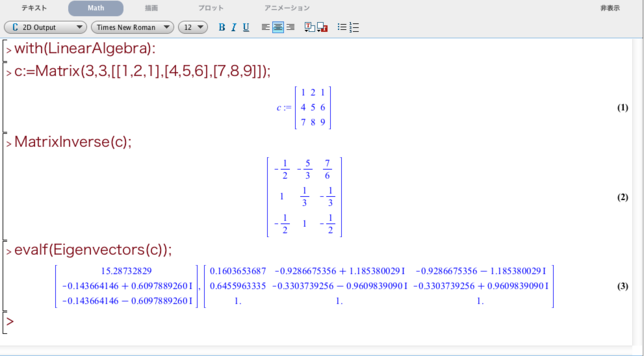
\includegraphics[width=10cm,bb= 0 0 737 553]{../figs/./mapleruby_eringi.exmaple.png}
\caption{Mapleの出力結果}
\label{default}\end{center}\end{figure}
よって正しく行列の計算ができた事が分かる.

